\documentclass[twocolumn]{IEEEtran11}


\usepackage[usenames,dvipnames]{xcolor} % for colored text
\usepackage[normalem]{ulem} % for strickthrough text

% quantum macros

\def\01{\{0,1\}}
\def\eps{\epsilon}
\newcommand{\half}{{\frac{1}{2}}}
\newcommand{\set}[1]{{\left\{#1\right\}}}
\newcommand{\ksubsets}{{n \choose k}}
\newcommand{\jsubsets}{{n \choose j}}
\newcommand{\Prob}{{\mathbf{Pr}}}
\newcommand{\tinyspace}{\mspace{1mu}}
\newcommand{\microspace}{\mspace{0.5mu}}
\newcommand{\op}[1]{\operatorname{#1}}

\newcommand{\norm}[1]{\left\lVert\tinyspace#1\tinyspace\right\rVert}
\newcommand{\snorm}[1]{\lVert\tinyspace#1\tinyspace\rVert}
\newcommand{\abs}[1]{\left\lvert\tinyspace #1 \tinyspace\right\rvert}
\newcommand{\ceil}[1]{\left\lceil #1 \right\rceil}
\newcommand{\floor}[1]{\left\lfloor #1 \right\rfloor}
\def\iso{\cong}
\newcommand{\defeq}{\stackrel{\smash{\text{\tiny def}}}{=}}
\newcommand{\tr}{\operatorname{tr}}
\newcommand{\rank}{\operatorname{rank}}
\renewcommand{\det}{\operatorname{Det}}
\newcommand{\im}{\operatorname{Im}}
\renewcommand{\t}{{\scriptscriptstyle\mathsf{T}}}
\newcommand{\ip}[2]{\left\langle #1 , #2\right\rangle}
\newcommand{\ipp}[1]{\left\langle #1 \right\rangle}
\newcommand{\sip}[2]{\langle #1 | #2\rangle}

\def\({\left(}
\def\){\right)}
\def\I{\mathsf{id}}

\newcommand{\fid}{\operatorname{F}}
\newcommand{\setft}[1]{\mathrm{#1}}
\newcommand{\lin}[1]{\setft{L}\left(#1\right)}
\newcommand{\density}[1]{\setft{Dens}\left(#1\right)}
\newcommand{\unitary}[1]{\setft{U}\left(#1\right)}
\newcommand{\trans}[1]{\setft{T}\left(#1\right)}
\newcommand{\herm}[1]{\setft{Herm}\left(#1\right)}
\newcommand{\pos}[1]{\setft{Pos}\left(#1\right)}
\newcommand{\pd}[1]{\setft{Pd}\left(#1\right)}
\newcommand{\sphere}[1]{\mathcal{S}\!\left(#1\right)}
\newcommand{\opset}[3]{\setft{#1}_{#2}\!\left(#3\right)}
\newcommand{\ot}{\otimes}

\def\complex{\mathbb{C}}
\def\real{\mathbb{R}}
\def\natural{\mathbb{N}}
\def\integer{\mathbb{Z}}

\def\<{\langle}
\def\>{\rangle}
\def \lket {\left|}
\def \rket {\right\rangle}
\def \lbra {\left\langle}
\def \rbra {\right|}
\newcommand{\ket}[1]{\lket\microspace #1 \microspace\rket}
\newcommand{\bra}[1]{\lbra\microspace #1 \microspace\rbra}
\newcommand{\ketbra}[1]{\lket\microspace #1 \rangle \langle #1 \microspace\rbra}


\def\X{\mathcal{X}}
\def\Y{\mathcal{Y}}
\def\Z{\mathcal{Z}}
\def\W{\mathcal{W}}
\def\A{\mathcal{A}}
\def\B{\mathcal{B}}
\def\V{\mathcal{V}}
\def\U{\mathcal{U}}
\def\C{\mathcal{C}}
\def\D{\mathcal{D}}
\def\H{\mathcal{H}}
\def\E{\mathcal{E}}
\def\F{\mathcal{F}}
\def\M{\mathcal{M}}
\def\R{\mathcal{R}}
\def\P{\mathcal{P}}
\def\Q{\mathcal{Q}}
\def\S{\mathcal{S}}
\def\T{\mathcal{T}}
\def\K{\mathcal{K}}
\def\yes{\text{yes}}
\def\no{\text{no}}
\def\onevec{\vec{\mathbf{1}}}

\newcommand{\trnorm}[1]{\norm{#1}_{\tr}}
\newcommand{\trnormb}[1]{{\big\| #1 \big\|}_{\rm tr}}
\newcommand{\trdist}[1]{ \left | #1 \right |_{\rm tr}}
\newcommand{\uniform}[1]{\mathcal{U}_{#1}}

\def\defeq{\stackrel{\small \textrm{def}}{=}}



\usepackage{amsmath}
\usepackage{epsfig}
\usepackage[T1]{fontenc}
\usepackage{graphicx}
\def\BibTeX{{\rm B\kern-.05em{\sc i\kern-.025em b}\kern-.08em
    T\kern-.1667em\lower.7ex\hbox{E}\kern-.125emX}}

\oddsidemargin -15pt
\evensidemargin -15pt
\leftmargin 0 pt
\topmargin -30pt
\textwidth = 6.9 in
\textheight = 9.0 in

\newcommand{\itembase}{\setlength{\itemsep}{0pt}}
\newcommand{\eg}{{\it e.g., }}
\newcommand{\ie}{{\it i.e., }}

% All the pretty colors go here
\definecolor{myGreen}{rgb}{0,1,0}
\definecolor{myRed}{rgb}{1,0,0}
\newcommand{\clb}{\color{blue}}
\newcommand{\clr}{\color{myRed}}
\newcommand{\clg}{\color{myGreen}}
\newcommand{\clbl}{\color{black}}

\begin{document}
\bibliographystyle{IEEE}

\title{{\Large \bf Cluster State Quantum Computing}\\ {\normalsize CIS:410/510 project proposal, Spring 2016}}
\author{
Dileep Reddy, Mayra Amezcua, Zach Schmidt \\
{\em dileep@uoregon.edu, mamezcua@cas.uoregon.edu, zschmidt@cs.uoregon.edu }
}
\maketitle

%\pagestyle{empty}
\begin{abstract}
Any quantum computation can be performed via sequences of one-qubit measurements on a specific type of initially entangled state -- the \textit{cluster state}. Each computational step is a projective measurement that destroys a quantum state, leaving a final state that relies on the outcomes of earlier computations. The model of interest is the one-way quantum computer which is based on this measurement scheme. This paper will present background regarding computation using only measurements, a brief introduction into the preparation of cluster states, a discussion of one way quantum computers (1WQC), and the computational power of various configurations of a 1WQC.
\end{abstract}

%\begin{keywords} 
%\end{keywords}

\section{Background}
Over the past few decades, advances in science and technology have greatly contributed to the development of modern computers. While these computers are efficient and convenient for everyday needs, they fail at certain computational tasks. Instead, quantum computers promise faster large scale factorization and database searches that are intractable for their classical counterparts. The first quantum computer designs were based off of classical models; sequences of one- and multi-qubit gate operations are performed on chosen quantum bits and a final measurement would convert quantum information into classical bits. A new model, proposed by Briegel and Raussendorf \cite{briegel2000measurements}, demonstrates that quantum computation can be achieved by using single qubit measurements as computational steps. This so-called cluster model or \textit{one-way quantum computer (1WQC)} relies on an entangled state of a large number of qubits or \textit{cluster state} as the resource. The fascinating feature about 1WQC is that they have no classical analogues and probe into new territory in regards to entanglement and measurements. 

\subsection{Cluster States}
Consider a set of qubits $\mathcal{C}$ labeled by an interger index, that are distributed in some lattice such that every qubit can be said to have adjacent neighbors. For these to collectively form a cluster state, their quantum mechanical state would be characterized by the set of eigenvalue equations \cite{briegel2001persistent},

\begin{equation}
  K_a\ket{\Phi}_{\mathcal{C}}= \kappa\ket{\Phi}_{\mathcal{C}}
\end{equation}

\noindent for a family of operators $K_a = X^{(a)}\bigotimes_{\gamma\in\Gamma(a)}Z^{(\gamma)}$, $a\in\mathcal{C}$, where $\Gamma(a)$ is the set of indices of all qubits in the ``adjacent neighborhood'' of $a$. The matrix $X^{(a)}$ is used to denote an $X$ operation on qubit-$a$, and so on. The eigenvalue $\kappa = \pm 1$ is determined by the specific occupation pattern of the neighboring sites. A method to prepare a one-dimensional cluster state is given in \cite{jorrand2005unifying}, consisting of ``cascading'' Controlled-$Z$ ($C_z$) gates on $n$ qubits, where:

\[
C_z = 
\begin{pmatrix}
  1 & 0 & 0 & 0 \\
  0 & 1 & 0 & 0 \\
  0 & 0 & 1 & 0 \\
  0 & 0 & 0 & -1 \\
 \end{pmatrix}
\]

The action of the $C_z$ gate in the computational basis can be seen to be $\ket{x,y} \to (-1)^{xy}\ket{x,y}$. Cluster states of arbitrary shape and connectivity can similarly be prepared via the recursive use of the Hadamard gate and two-qubit fusion operations \cite{browne2005efficient,gerald2006efficient}. Analogously, a large cluster state can be arbitrarily trimmed, split, and/or reshaped by removing qubits from the cluster. This is accomplished by measuring the target qubit in the computational basis, and performing appropriate unitary rotations on its erstwhile neighbors based on the measurement outcome. Intuitively, a cluster state can be thought of as a graph where every vertex represents a qubit, and every edge represents the application of a $C_z$ gate to both adjacent vertices.

\begin{figure}[thb]
  \centering
  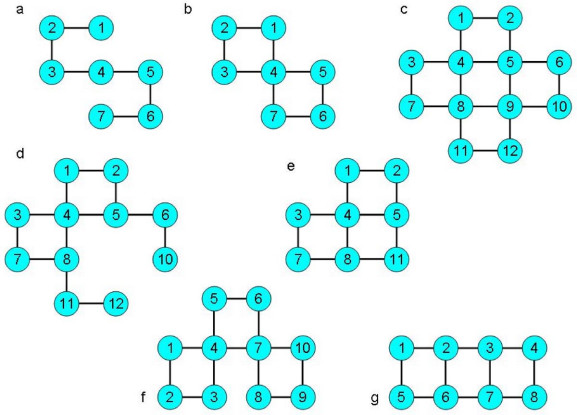
\includegraphics[width=0.9\linewidth]{2d_clusters_rep.jpg}
  \label{2dclustersfig}
  \caption{Figure from \protect\cite{gerald2006efficient}, showing representative 2-D cluster shapes. The vertices are qubits with integer indices, and the edges indicate entanglement connectivity between select neighbors.}
\end{figure}

Briegel and Raussendorf show that any quantum logic circuit can be implemented on a cluster state, which demonstrates universality of the proposed scheme \cite{briegel2000measurements}. Nielsen \cite{nielsen108020universal} extended this result to no longer require coherent dynamics, instead relying on a method to teleport quantum gates, and he provided a concise algorithm to accomplish this. 

\subsection{One-Way Quantum Computation}
All quantum computation schemes may be characterized by some combination of state preparation, unitary transformation of said states, and measurements on the same. Human-usable computational tasks necessarily require both input and final output to be classical information. The classical input information can influence the quantum computation in choice of initial states, the choice of unitary transforms (\ie algorithm), and the choice of measurement bases. The output is always a classical function of the measurement outcomes. In typical models for quantum computation, entire algorithms are implemented as a sequence of unitary transformations on a prepared quantum state (stored in qubits) of size appropriate to the problem, with a round of measurements as the final step. In such models, the unitary transformation stage is completely reversible. The splitting of the effective unitary matrix into sequential steps can be arbitrary and entirely dependent on physical hardware limitations. There is no correspondence with ``computational steps'' or ``clock cycles'' in the classical sense, as the quantum state of the computer in the midst of the unitary stages is inaccessible for diagnosis or debugging purposes. Any leakage of information into computer memory or environment constitutes decoherence, and will introduce errors in the computation.

One-way quantum computation, on the other hand, revolves around single qubit measurements as a progression of computational steps. Measurements are a crucial component to quantum information processing because they irreversibly destroy a quantum state. Entanglement, on the other hand, will ensure that the state of the final qubit relies on the outcomes of preceding measurements. Given a cluster state, a series one-qubit measurements can be performed at each qubit to implement a quantum gate \cite{jorrand2005unifying}.  The unidirectionality of cluster state computation is inherent, due to the fact that quantum information cannot be accurately recovered once a measurement has been made. Consider a two-dimensional array of entangled qubits, information propagates horizontally through a row of qubits while vertical qubit neighbors are used for two-qubit gates. Similarly, three-dimensional clusters can be used to implement topologically protected gates \cite{raussendorf2007topological}, where the gate function only depends upon the way ``connected defects'' are wound around one another, but not on the details of their shape. This degree of freedom affords the design some fault tolerance.

\subsection{Computational Power and Complexity}
The spacial layout of the graph representation of the cluster state plays a role in the computational power of that state. If a cluster state can be prepared linearly via the cascading $C_z$ technique mentioned above, it can be represented as a  ``one-dimensional'' graph (i.e., some graph $G=(V,E),\ \forall v\in V$, deg$(v)\leq 2$). A linearly prepared cluster state can be efficiently simulated on a classical computer in $O(n\log ^c (1/n))$, where $n$ is the initial number of qubits, and $c$ is the cost of floating point multiplication \cite{nielsen2006cluster}. Though the author consequently dismisses linearly prepared cluster states as a substrate for quantum computation, it would be interesting to know which class of problems they would be able to solve. \\
In general, measurement based models can be polynomial time reduced to the gate array model, and thus have the same power, but they are more easily parallelizable \cite{jozsa2006introduction}.\\
The gate teleportation algorithm \cite{nielsen108020universal} has a time complexity of $O(\log (1/\epsilon))$, where $\epsilon$ is the failure probability. 

\section{Proposal}

This project will attempt to discuss some background on cluster states, a correspondence between 1WQC and the more traditional gate array model, and the computational power of this new model. We aim to review the literature surrounding 1WQCs and cluster states. We shall present the concept as an extension of basic quantum teleportation. Additionally, we will focus on the complexity and universality of this model and explore the physical implementations of cluster states, with special emphasis on optics related technologies. We will illustrate possible advantages and disadvantages cluster states have in contrast to other approaches. If time permits, we also intend to explore fault-tolerant cluster state schemes, and the implications of cluster states with qudits.


%% file citations.bib contains all the biblography
\bibliography{citations}
\end{document}
